% Report for the DSL504 course project (Group 10). Build from this folder:
%   pdflatex report.tex && pdflatex report.tex
% Every number comes from a results file in ../results/ and the run table in ../logs.md (Appendix A).
\documentclass[11pt,a4paper]{article}

% ---------- fonts and page ----------
\usepackage[T1]{fontenc}
\usepackage[utf8]{inputenc}
\usepackage[sc]{mathpazo}
\linespread{1.06}
\usepackage[scaled=0.92]{helvet}
\renewcommand{\ttdefault}{lmtt}
\usepackage[a4paper,margin=2.4cm,headheight=15pt]{geometry}
\usepackage{microtype}

% ---------- tools ----------
\usepackage{graphicx}
\usepackage{booktabs}
\usepackage{tabularx}
\usepackage{array}
\usepackage{amsmath}
\usepackage{xcolor}
\usepackage{enumitem}
\usepackage{caption}
\usepackage{listings}
\usepackage{float}
\usepackage{titlesec}
\usepackage{fancyhdr}
\usepackage{lastpage}
\usepackage{tcolorbox}
\usepackage{needspace}
\usepackage[titles]{tocloft}
\setlength{\cftbeforesecskip}{3pt}
\tcbuselibrary{skins}

% ---------- colours ----------
\definecolor{brand}{RGB}{23,54,93}
\definecolor{brandlight}{RGB}{232,239,247}
\definecolor{muted}{gray}{0.42}
\definecolor{codebg}{gray}{0.965}

\PassOptionsToPackage{hyphens}{url}
\usepackage[colorlinks=true,linkcolor=brand,urlcolor=brand,citecolor=brand]{hyperref}

% ---------- headings ----------
\titleformat{\section}{\sffamily\Large\bfseries\color{brand}}{\thesection}{0.7em}{}[{\color{brand!25}\titlerule[0.6pt]}]
\titleformat{\subsection}{\sffamily\large\bfseries\color{brand!85!black}}{\thesubsection}{0.6em}{}
\newcommand{\sectionbreak}{\needspace{8\baselineskip}}
\titlespacing*{\section}{0pt}{18pt plus 4pt minus 2pt}{8pt}
\titlespacing*{\subsection}{0pt}{12pt plus 3pt minus 2pt}{4pt}

% ---------- headers and footers ----------
\fancypagestyle{main}{%
  \fancyhf{}%
  \fancyhead[L]{\sffamily\small\color{muted}Indian Address Parser}%
  \fancyhead[R]{\sffamily\small\color{muted}DSL504 \textperiodcentered\ Group 10}%
  \fancyfoot[C]{\sffamily\small\color{muted}Page \thepage\ of \pageref{LastPage}}%
  \renewcommand{\headrulewidth}{0.4pt}%
  \renewcommand{\headrule}{\hbox to\headwidth{\color{brand!30}\leaders\hrule height \headrulewidth\hfill}}}
\fancypagestyle{front}{%
  \fancyhf{}%
  \fancyfoot[C]{\sffamily\small\color{muted}\thepage}%
  \renewcommand{\headrulewidth}{0pt}}
\fancypagestyle{plain}{%
  \fancyhf{}%
  \fancyfoot[C]{\sffamily\small\color{muted}\thepage}%
  \renewcommand{\headrulewidth}{0pt}}

% ---------- captions, lists, code, boxes ----------
\captionsetup{font=small, labelfont={bf,sf,color=brand}, skip=6pt}
\setlist{itemsep=2pt, topsep=4pt}
\setlength{\parskip}{4pt}
\lstset{basicstyle=\ttfamily\small, backgroundcolor=\color{codebg}, frame=l, framerule=2pt, rulecolor=\color{brand!55},
  breaklines=true, columns=fullflexible, keepspaces=true, aboveskip=7pt, belowskip=7pt, xleftmargin=6pt,
  framexleftmargin=6pt, upquote=true}
\newtcolorbox{keybox}[1]{enhanced, colback=brandlight, colframe=brand, boxrule=0.6pt, arc=2pt,
  fonttitle=\sffamily\bfseries, title=#1, before upper={\raggedright}, left=8pt, right=8pt, top=6pt, bottom=6pt}
\newtcolorbox{notebox}{enhanced, colback=gray!6, colframe=gray!55, boxrule=0.5pt, arc=2pt,
  left=8pt, right=8pt, top=5pt, bottom=5pt}
\newcolumntype{L}{>{\raggedright\arraybackslash}X}
\newcommand{\code}[1]{\texttt{#1}}

\begin{document}

% ======================= title page =======================
\pagenumbering{Alph}
\begin{titlepage}
\centering
{\sffamily\large\color{brand}INDIAN INSTITUTE OF TECHNOLOGY BHILAI\par}
\vspace{4pt}
{\sffamily\color{muted}DSL504 \textperiodcentered\ Natural Language Processing\par}
\vspace{2.6cm}
{\color{brand}\rule{\linewidth}{1.2pt}\par}
\vspace{16pt}
{\sffamily\fontsize{30}{36}\selectfont\bfseries\color{brand}Indian Address Parser\par}
\vspace{12pt}
{\LARGE Parsing and Normalising Messy Indian Addresses\par}
\vspace{16pt}
{\color{brand}\rule{\linewidth}{1.2pt}\par}
\vspace{12pt}
{\large\itshape Course Project Report\par}
\vspace{2.6cm}
{\sffamily\large\bfseries\color{brand}Group 10\par}
\vspace{10pt}
{\large
\begin{tabular}{@{}l@{\hspace{3em}}l@{}}
\toprule
\textsf{\textbf{Name}} & \textsf{\textbf{Reg.\ No.}}\\
\midrule
Agastya Nath & 12340140\\
Paritosh Lahre & 12341550\\
Varun Rao & 12342320\\
Y. Rahul Dev Reddy & 12342390\\
\bottomrule
\end{tabular}\par}
\vfill
{\small
\begin{tabular}{@{}r@{\hspace{1em}}l@{}}
\textsf{\color{muted}Project duration} & October--November 2026\\
\textsf{\color{muted}Submitted} & 16 November 2026\\
\textsf{\color{muted}Code} & \url{https://github.com/devreddy1015/NLP_GROUP_PROJECT}\\
\textsf{\color{muted}Model} & \url{https://huggingface.co/sandstromPL/muril-indian-address-parser}\\
\end{tabular}\par}
\end{titlepage}

% ======================= front matter =======================
\pagestyle{front}
\pagenumbering{roman}

\section*{Abstract}
People in India write addresses in many styles: with landmarks (``behind SBI ATM''), short forms (``b'lore-68''),
Hindi words in English letters (``hanuman mandir ke paas''), in any order and often without commas. We built a system
that labels each word of such an address with one of nine fields (house, building, street, landmark, locality, city,
district, state and PIN), cleans the fields, and checks the PIN against the India Post directory of 157,126 post
offices. Because real labelled addresses are rare, we wrote a program that makes 20,000 practice (synthetic) addresses
with eight kinds of realistic mistakes, and trained a rules system, a CRF and two transformer models (MuRIL and \mbox{XLM-R})
on them. On 2,000 new synthetic addresses the trained models score 0.991--0.992 F1, but on 20 addresses written by hand
they score only 0.741--0.796, while the simple rules score 0.828. On the same 20 addresses, every one of our systems
beats five existing open-source Indian address parsers and a small language model. We also ran the model on 20 more
test addresses (13 real addresses of public offices and 7 invented hard cases) to see where it fails. A larger test set
of about 500 human-written addresses was planned but not collected before the deadline, so our main question is only
partly answered.

\medskip
\noindent\textsf{\textbf{\color{brand}Keywords:}} sequence labelling, address parsing, Indian addresses, synthetic
data, MuRIL, CRF, PIN code checking

\bigskip
\begin{keybox}{Results at a glance}
\begin{itemize}[leftmargin=1.2em, itemsep=3pt]
\item \textbf{Task:} label every word of an Indian address with one of nine fields, then check the PIN against
157,126 India Post offices.
\item \textbf{Training data:} 20,000 synthetic addresses with eight kinds of realistic noise.
\item \textbf{Synthetic test (2,000 addresses):} CRF 0.992, \mbox{XLM-R} 0.991, MuRIL 0.991 span F1.
\item \textbf{20 hand-written addresses:} rules 0.828, CRF 0.796, \mbox{XLM-R} 0.759, MuRIL 0.741 span F1.
\item \textbf{Against existing parsers:} all 28 comparisons (our 4 systems against 7 others) are clearly in our
favour.
\item \textbf{Public model:} \url{https://huggingface.co/sandstromPL/muril-indian-address-parser}
\end{itemize}
\end{keybox}

\clearpage
\setcounter{tocdepth}{1}
\tableofcontents
\listoftables
\listoffigures
\clearpage

% ======================= main text =======================
\pagestyle{main}
\pagenumbering{arabic}

\section{Introduction}

\subsection{The problem}
In India, people rarely write an address in one fixed format. A typical address looks like this:
\begin{lstlisting}
opp. ganesh temple, 2nd cross, behind old bus stand, hosur road, madivala, b'lore-68
\end{lstlisting}
It uses two landmarks (``opp.\ ganesh temple'', ``behind old bus stand''), short forms (``opp.'', ``b'lore'') and only
the last two digits of the PIN (``68''). Other addresses use Hindi words written in English letters (``hanuman mandir
ke paas'' means ``near the Hanuman temple''), leave out commas, or put the parts in any order.

Delivery companies, banks and emergency services need addresses as separate, clean fields: house, street, locality,
city, PIN and so on. Turning free text into such fields is a classic NLP task called \emph{sequence labelling}: we give
every word a label. India Post's new DIGIPIN gives every small square of land a code, but people will keep writing
addresses in words, so this problem stays useful.

\subsection{What we built}
\begin{enumerate}
\item A \textbf{tagger} that labels every word of an address with one of nine fields (Section~\ref{sec:task}).
\item A \textbf{normaliser} that cleans the fields (it expands short forms and splits each landmark into a relation
and a place) and checks the PIN against the India Post directory.
\item A small \textbf{web demo}: type an address and see the tagged parts, the cleaned fields and the PIN check.
\end{enumerate}

\subsection{Our research question}
Real Indian addresses with correct labels are hard to get, partly because of privacy. So most address parsers,
including ours, are trained on \emph{synthetic} addresses that a program writes. Such models score almost perfectly on
more synthetic addresses. We asked:
\begin{itemize}
\item \textbf{RQ1 (the gap):} how much worse do these models do on addresses that people actually write?
\item \textbf{RQ2 (which noise helps):} which kinds of realistic mistakes, added to the synthetic data, close the
gap most?
\item \textbf{RQ3 (real data):} how much does adding a few real labelled addresses help?
\end{itemize}

\subsection{What we found}
\begin{itemize}
\item On 2,000 new synthetic addresses, our trained models score 0.991--0.992 F1 (F1 is a score from 0 to 1,
explained in Section~\ref{sec:measure}).
\item On 20 addresses written by hand, they score 0.741--0.796. A simple rule-based system scores 0.828.
\item On the same 20 addresses, all our systems beat five existing open-source Indian address parsers and a small
language model, and the differences are clear (their 95\,\% intervals do not include zero).
\item We planned to collect about 500 real addresses for the main test but did not collect them before the
deadline. So RQ1 is answered only on a small set, and RQ2 and RQ3 are left for future work.
\end{itemize}

\section{Related work}
\textbf{The closest work} is by Dhavase and Chaudhary (2026)~\cite{etasr}. They trained four transformer models
(IndicBERT, MuRIL, DeBERTa-v3 and \mbox{XLM-R}) on 15,000 addresses made by a grammar, with no spelling mistakes or short
forms. The models scored 0.989--0.995 F1 on synthetic test data, but dropped sharply on 500 addresses built from
OpenStreetMap: \mbox{XLM-R}, for example, scored 0.006 on house numbers and 0.011 on roads. They closed part of the gap by
looking up each predicted part in a list of place names. Their labels have no landmark, and their ``real'' test set
was made by a script, not written by people.

\textbf{Open models.} Several models for Indian addresses are free on Hugging Face: two Shiprocket models (IndicBERT
and TinyBERT), a MuRIL model by mukuls9971, a TinyBERT model by gagan1985, and a 1.5-billion-parameter model by
abr-6024 that answers in JSON~\cite{shiprocket,mukuls,gagan,abr}. We ran these five on our hand-written addresses
without any training.

\textbf{Other work.} General address parsers such as deepparse~\cite{deepparse} and libpostal are trained mostly on
other countries' addresses. Companies that deliver parcels in India work on this problem (for example
GeoIndia~\cite{geoindia}), but they keep their data private. We found no public dataset of real, human-written Indian
addresses with labels.

\textbf{How we differ.} (1) We test on addresses written by people. (2) We have a LANDMARK label. (3) We try to close
the gap by improving the training data (realistic mistakes plus a few real examples) instead of adding a lookup step.

\section{The task}\label{sec:task}
Each address is split into words, and every punctuation mark is its own word. Each word gets a label from
Table~\ref{tab:labels}.

\begin{table}[H]
\centering\small
\caption{The nine fields.}\label{tab:labels}
\begin{tabularx}{\textwidth}{lLL}
\toprule
\textbf{Field} & \textbf{What it covers} & \textbf{Examples}\\
\midrule
HOUSE & house, flat, plot, shop or door number; floor & Flat 3B, H.No.\ 12/3, Shop No.\ 4, 2nd floor\\
BUILDING & apartment, society, complex, named building & Shanti Apts, Surya Mall, Tower C\\
STREET & road, street, lane, cross, main, gali, highway & MG Road, 2nd cross, Gali No.\ 4, NH 44\\
LANDMARK & a relation word and the landmark & near Hanuman Mandir, opp.\ petrol pump, SBI ATM ke paas\\
LOCALITY & area, colony, nagar, sector, village & Supela, Sector 21, Koramangala 4th Block\\
CITY & city or town, in any spelling & Bhilai, B'lore, Hyd\\
DISTRICT & district, only next to a word like Dist or Zila & Durg in ``Distt.\ Durg''\\
STATE & state or union territory, also short forms & Chhattisgarh, C.G., MH\\
PIN & the 6-digit PIN, also spaced or partial & 490023, 490 023, 68 in b'lore-68\\
\bottomrule
\end{tabularx}
\end{table}

We use \textbf{BIO tags}: \code{B-} marks the first word of a part, \code{I-} marks the next words of the same part,
and \code{O} marks words that belong to no part. For example:
\begin{lstlisting}
shanti/B-BUILDING  apts/I-BUILDING  ,/O
behind/B-LANDMARK  SBI/I-LANDMARK  atm/I-LANDMARK
\end{lstlisting}
A few rules keep the labels consistent. The relation word (\emph{near}, \emph{opp.}, \emph{behind}) belongs to the
LANDMARK. The name of the place the address is for (``Shree Sweets'', ``IIT Bhilai'') gets \code{O}. A district name
gets DISTRICT only when a word like \emph{Dist} or \emph{Zila} is next to it; otherwise it is a CITY.

\section{Data}

\subsection{The India Post PIN directory}
The All India Pincode Directory (data.gov.in) lists 157,126 post offices with their PIN, district and state: 19,300
PINs in 36 states and union territories. We clean the names (for example, \code{C.G.}, \code{CG} and
\code{Chattisgarh} all become Chhattisgarh) and use the directory in three places: to build synthetic addresses, as
extra knowledge for the rules and the CRF, and to check PINs.

\subsection{Synthetic addresses}
Our generator fills address templates with real places from the PIN directory. Because the program writes the
address, it knows the correct label of every word, so the labels are free. On top of a clean address it adds eight
kinds of realistic noise (Table~\ref{tab:noise}). Each kind can be switched off, which is how RQ2 would be tested.

\begin{table}[H]
\centering\small
\caption[The eight kinds of noise]{The eight kinds of noise in the synthetic addresses.}\label{tab:noise}
\begin{tabularx}{\textwidth}{llL}
\toprule
\textbf{ID} & \textbf{Noise} & \textbf{Examples}\\
\midrule
N1 & Short forms & Road $\rightarrow$ Rd, Apartments $\rightarrow$ Apts, near $\rightarrow$ nr, Bangalore
$\rightarrow$ B'lore, Chhattisgarh $\rightarrow$ CG\\
N2 & Landmark phrases & opposite / behind / next to X; X ke paas, X ke samne (Hinglish); 0, 1 or 2 landmarks\\
N3 & Dropped or reordered fields & a field left out (never the PIN), landmarks first, city and locality swapped\\
N4 & Separators and case & spaces, dashes or slashes instead of commas; all lower case or ALL CAPS\\
N5 & Typos & one or two letters added, removed, changed or swapped (never in the PIN)\\
N6 & Spelling variants & Mandir $\rightarrow$ Mandeer, Gali $\rightarrow$ Galli, Station $\rightarrow$ Steshan\\
N7 & PIN variants & 490 023, 490-023, ``Pin: 490023'', Bhilai-23, no PIN\\
N8 & House-number formats & \#12, H.No 12/3, D.No 5-6-7/A, Flat No.\ 3B, Khasra No 12\\
\bottomrule
\end{tabularx}
\end{table}

With all eight kinds switched on (the \code{full} set), we made 20,000 training, 2,000 dev and 2,000 test addresses.
The PINs were split 90/5/5 first, so dev and test addresses use PINs that the model never saw in training.

\subsection{hand20: 20 addresses written by hand}
For a first look at real text, the team wrote 20 addresses of public places by hand and labelled them (94 parts in
total). 17 are from Bhilai, Durg and Raipur, and one each from Bengaluru, Madurai and Mumbai; one is in Devanagari.
This set is small, and the team also used it while building the system, so its scores are a rough check, not a final
result.

\subsection{The planned real test set}
The main test was to be about 500 addresses written by classmates and friends in a Google Form: addresses of public
places (shops, temples, colleges, hospitals, offices) written as they would write them for a courier, and never a
home address, a name or a phone number. The plan was 250 for testing, 50 for development and 200 as real training
data for RQ3, with two people labelling the same 50 to measure how much they agree. The form, the labelling guide and
all the tools are ready, but the form was not sent before the deadline.

\section{Our systems}

\subsection{Rules}
A hand-written baseline. It splits the address at commas, finds the PIN with a pattern (six digits), starts a
landmark at words like \emph{near}, \emph{opp.} or \emph{behind}, and uses word lists (Road, Nagar, Apartments,
Dist, \ldots) and the PIN directory to label the rest. It needs no training.

\subsection{CRF}
A conditional random field is a classic model for sequence labelling. For each word it looks at simple features (the
word itself, its last letters, whether it is a number or looks like a PIN, whether it is a known city or a cue word
such as \emph{Road}) and at the same features of the two words on each side. It then picks the best sequence of tags
for the whole address.

\subsection{MuRIL and XLM-R}
Both are pre-trained transformer models, like BERT. MuRIL~\cite{muril} was built by Google for Indian languages and
was also trained on Indian text written in English letters, which suits Hinglish. \mbox{XLM-R}~\cite{xlmr} is a multilingual
model and the strongest model in the closest work. \emph{Fine-tuning} means we add a small layer that predicts one of
19 tags (\code{O}, plus \code{B-} and \code{I-} for each of the nine fields) for each word, and then train the whole
model on our 20,000 synthetic addresses. A word can be split into several smaller pieces; we use the prediction for
the first piece.

\textbf{Training settings.} 3 passes over the data (epochs), learning rate $10^{-4}$, 32 addresses per step, warm-up
over the first 10\,\% of steps, weight decay 0.01, gradient clipping 1.0, 16-bit (bf16) mixed precision, at most 256
pieces per address, random seed 42. We chose these on 11 November from five MuRIL runs (Table~\ref{tab:tuning}), with
a rule set before the runs: take the cheapest setting within 0.002 F1 of the best score on synthetic dev. The model in
our demo was trained with these settings on 16 November in 357 seconds on an RTX 4060 laptop GPU (8\,GB); its average
loss per epoch fell from 1.476 to 0.138 to 0.053. It has about 237 million parameters and is public on Hugging Face.

\subsection{Existing open parsers}
We ran the five open models from Section 2 as they are. Their labels differ from ours (for example, Shiprocket's
\code{house\_details} and \code{floor} both mean our HOUSE), so we map their labels onto ours and score each one only
on the labels it shares with us.

\subsection{A small language model}
We asked Qwen2.5-1.5B-Instruct~\cite{qwen} to return our nine fields as JSON. In one run the prompt had no examples;
in the other it had 5 example addresses with their answers (this is called \emph{in-context learning}). The examples
were synthetic, because we had no real ones.

\subsection{The normaliser}
It expands short forms (\code{Apts} $\rightarrow$ Apartments, \code{b'lore} $\rightarrow$ Bangalore), splits each
landmark into a relation (\emph{behind}) and a place (\emph{SBI atm}), and checks the PIN. The PIN check gives one of
four answers: \emph{valid}, \emph{mismatch} (the PIN belongs to a different state or district than the one written),
\emph{not found} (the PIN is not in the directory), or \emph{missing}. When the PIN is valid, it fills in a missing
district and state.

\section{How we measure}\label{sec:measure}
\textbf{Precision} is the share of the parts a system found that are right. \textbf{Recall} is the share of the true
parts that the system found. \textbf{F1} combines the two:
\[
F_1 = \frac{2 \times \text{precision} \times \text{recall}}{\text{precision} + \text{recall}}
\]
\begin{itemize}
\item \textbf{Span F1} (our main score): a part counts as right only if its words and its label are both exactly
right. We use the \code{seqeval} library in strict mode. ``Micro'' F1 counts all parts together; ``macro'' F1 is the
average over the nine fields.
\item \textbf{Field F1}: compares the cleaned text of each field. We use it for the systems that answer in JSON,
because they do not tag words.
\item \textbf{Exact match}: the share of addresses in which every tag is right.
\item \textbf{95\,\% confidence interval}: we draw the test addresses again at random, 1,000 times (a
\emph{bootstrap}), and see how much the score moves. With only 20 addresses, the intervals are wide.
\item \textbf{Comparing two systems}: we use a \emph{paired} bootstrap on the same addresses. If the interval of the
difference does not include zero, we call the difference clear.
\end{itemize}
To be fair, every number below comes from a results file in the project (\code{results/}), and each run is listed in
the project's work log (\code{logs.md}); Appendix~\ref{app:runs} gives the run behind each table.

\section{Results}

\subsection{Synthetic addresses against hand-written ones}
\begin{table}[H]
\centering\small
\caption[Main results: synthetic dev and hand20]{Span F1 (micro) with 95\,\% intervals. Dev = 2,000 synthetic addresses with unseen PINs; hand20 = 20
hand-written addresses. Exact match is the share of hand20 addresses tagged completely right.}\label{tab:main}
\begin{tabular}{lccc}
\toprule
\textbf{System} & \textbf{Synthetic dev} & \textbf{hand20} & \textbf{Exact match}\\
\midrule
Rules (no training) & -- & 0.828 (0.745--0.897) & 0.250\\
CRF & 0.992 (0.990--0.993) & 0.796 (0.708--0.889) & 0.400\\
\mbox{XLM-R}, fine-tuned & 0.991 (0.989--0.993) & 0.759 (0.677--0.840) & 0.350\\
\textbf{MuRIL, fine-tuned} & \textbf{0.991 (0.989--0.992)} & \textbf{0.741 (0.645--0.830)} & \textbf{0.350}\\
\bottomrule
\end{tabular}
\end{table}

All three trained models are almost perfect on synthetic addresses: MuRIL tags 1,891 of the 2,000 dev addresses
completely right. On hand-written addresses they lose between 0.20 and 0.25 F1. This is the gap that RQ1 asks about,
seen on a small set.

\begin{notebox}
\textbf{\textsf{Read with care.}} The simple rules score best on hand20, but the intervals of all four systems overlap,
so 20 addresses are not enough to rank them. The rules were also written with these 20 addresses in view.
\end{notebox}

\subsection{Existing parsers}
\begin{table}[H]
\centering\small
\caption[Existing open parsers on hand20]{Existing open parsers on hand20, used as they are. The taggers are scored only on the labels they share with
us; the JSON systems at field level.}\label{tab:existing}
\begin{tabular}{lcc}
\toprule
\textbf{System} & \textbf{Span F1 (95\,\% interval)} & \textbf{Field F1}\\
\midrule
Shiprocket IndicBERT & 0.588 (0.489--0.684) & 0.591\\
Shiprocket TinyBERT & 0.469 (0.365--0.579) & 0.480\\
mukuls9971 MuRIL NER & 0.418 (0.355--0.500) & 0.420\\
gagan1985 TinyBERT & 0.386 (0.316--0.466) & 0.386\\
abr-6024 parser (1.5B, JSON) & -- & 0.645\\
Qwen2.5-1.5B, 5 examples (JSON) & -- & 0.484\\
Qwen2.5-1.5B, no examples (JSON) & -- & 0.288\\
\bottomrule
\end{tabular}
\end{table}

None of the four existing taggers tags any of the 20 addresses completely right (exact match 0.000). With no examples,
the language model gave valid JSON for only 9 of the 20 addresses; five synthetic examples fixed that (20 of 20).

\subsection{Our systems against existing parsers}
Table~\ref{tab:compare} compares MuRIL with each existing system on the labels they share, using that system's own
scoring rules and a paired bootstrap over the same 20 addresses. The rules, the CRF and \mbox{XLM-R} give the same picture:
all 28 comparisons (4 of our systems against 7 others) are clearly in our favour. Part of the margin comes from
conventions rather than parsing: the existing models tag the name of the place itself as a building or house, which
our labels leave out, and the abr-6024 model answers ``4'' for ``shop no 4'' and drops the relation word of a
landmark.

\begin{table}[H]
\centering\small
\caption[MuRIL against the existing parsers]{Field F1 on shared labels, hand20. Difference = MuRIL minus the other system, with its 95\,\% interval.}
\label{tab:compare}
\begin{tabular}{lccc}
\toprule
\textbf{Existing system} & \textbf{Its F1} & \textbf{MuRIL on the same labels} & \textbf{Difference}\\
\midrule
abr-6024 parser 1.5B & 0.645 & 0.791 & +0.147 (+0.033 to +0.249)\\
Shiprocket IndicBERT & 0.591 & 0.768 & +0.176 (+0.083 to +0.278)\\
Qwen2.5-1.5B, 5 examples & 0.484 & 0.768 & +0.285 (+0.183 to +0.387)\\
Shiprocket TinyBERT & 0.480 & 0.768 & +0.287 (+0.172 to +0.403)\\
mukuls9971 MuRIL NER & 0.420 & 0.768 & +0.346 (+0.247 to +0.452)\\
gagan1985 TinyBERT & 0.386 & 0.780 & +0.388 (+0.319 to +0.461)\\
Qwen2.5-1.5B, no examples & 0.288 & 0.768 & +0.481 (+0.391 to +0.598)\\
\bottomrule
\end{tabular}
\end{table}

\subsection{Field by field}
\begin{table}[H]
\centering\small
\caption[Span F1 per field]{Span F1 per field. ``Parts'' is the number of true parts of that field.}\label{tab:perlabel}
\begin{tabular}{lrcrcccc}
\toprule
& \multicolumn{2}{c}{\textbf{Synthetic dev}} & \multicolumn{5}{c}{\textbf{hand20}}\\
\cmidrule(lr){2-3}\cmidrule(lr){4-8}
\textbf{Field} & \textbf{Parts} & \textbf{MuRIL} & \textbf{Parts} & \textbf{Rules} & \textbf{CRF} & \textbf{\mbox{XLM-R}} &
\textbf{MuRIL}\\
\midrule
HOUSE & 1,577 & 1.000 & 4 & 1.000 & 0.400 & 0.500 & 0.571\\
BUILDING & 1,611 & 1.000 & 3 & 1.000 & 0.800 & 0.500 & 0.500\\
STREET & 1,621 & 0.999 & 11 & 1.000 & 0.615 & 0.800 & 0.714\\
LANDMARK & 2,235 & 0.999 & 7 & 0.923 & 0.923 & 0.667 & 0.667\\
LOCALITY & 1,609 & 0.959 & 17 & 0.562 & 0.703 & 0.606 & 0.588\\
CITY & 1,637 & 0.969 & 20 & 0.788 & 0.927 & 0.824 & 0.778\\
DISTRICT & 1,586 & 0.994 & 3 & 0.571 & 0.400 & 0.400 & 0.400\\
STATE & 1,589 & 0.994 & 13 & 0.818 & 0.815 & 0.800 & 0.815\\
PIN & 1,623 & 1.000 & 16 & 0.968 & 0.938 & 1.000 & 1.000\\
\bottomrule
\end{tabular}
\end{table}

The PIN is the most reliable field, even on hand-written text (0.938--1.000 for all four systems). Among the fields
that appear often in hand20, LOCALITY is the hardest for the rules, \mbox{XLM-R} and MuRIL, and the CRF's second hardest after
STREET. LOCALITY and CITY are often confused with each other (Section~\ref{sec:errors}). HOUSE, BUILDING and DISTRICT
have only 3 or 4 parts each in hand20, too few to say anything about them.

\subsection{Training settings and cost}
\begin{table}[H]
\centering\small
\caption[MuRIL training settings and cost]{MuRIL with different settings (synthetic \code{full}, seed 42, RTX 4060 laptop GPU; lr = learning rate). The
settings were chosen on synthetic dev only; hand20 is shown for interest.}\label{tab:tuning}
\begin{tabular}{llccc}
\toprule
\textbf{Setting} & \textbf{Precision} & \textbf{Synthetic dev F1} & \textbf{hand20 F1} & \textbf{Training time}\\
\midrule
3 epochs, lr $5\times10^{-5}$ (first try) & 32-bit & 0.988 & 0.745 & 508 s\\
3 epochs, lr $5\times10^{-5}$ & bf16 & 0.983 & 0.783 & 318 s\\
5 epochs, lr $5\times10^{-5}$ & bf16 & 0.991 & 0.777 & 527 s\\
\textbf{3 epochs, lr $10^{-4}$ (chosen)} & bf16 & 0.990 & 0.737 & 314 s\\
3 epochs, lr $10^{-4}$ & 32-bit & 0.990 & 0.777 & 532 s\\
5 epochs, lr $10^{-4}$ & bf16 & 0.990 & 0.768 & 523 s\\
Chosen, trained again (demo model) & bf16 & 0.991 & 0.741 & 357 s\\
\bottomrule
\end{tabular}
\end{table}

Mixed precision (bf16) gives the same synthetic score as 32-bit precision and trains 1.7 times faster. \mbox{XLM-R} with the
same settings took 361 s and used 7.2 of the GPU's 8.2\,GB, so a 4\,GB laptop GPU cannot train these models, though
it can run them. One warning sign: two runs that differ only in precision score the same on synthetic dev (0.990) but
0.737 and 0.777 on hand20. With 20 addresses, scores move this much between runs, which is why the plan asks for
three seeds and a larger test set.

\subsection{The PIN check}
\begin{table}[H]
\centering\small
\caption[PIN check results]{PIN check results. On synthetic dev and hand20 the normaliser was run on the correct tags; on the 20 test
cases (Section~\ref{sec:stress}) it was run on MuRIL's tags.}\label{tab:pin}
\begin{tabular}{lrrrrr}
\toprule
\textbf{Addresses} & \textbf{Count} & \textbf{Valid} & \textbf{Missing} & \textbf{Not found} & \textbf{Mismatch}\\
\midrule
Synthetic dev & 2,000 & 1,376 & 377 & 244 & 3\\
hand20 & 20 & 15 & 4 & 1 & 0\\
Test cases: real public offices & 13 & 4 & 0 & 1 & 8\\
Test cases: invented & 7 & 0 & 0 & 7 & 0\\
\bottomrule
\end{tabular}
\end{table}
On synthetic dev, every district (249 of 249) and every state (287 of 287) that the normaliser filled in from a valid
PIN was right.

\section{Examples and error analysis}\label{sec:errors}

\subsection{Three examples}
These are real outputs of the MuRIL model and the normaliser, as the demo shows them.

\noindent{\sffamily\bfseries\color{brand}Example 1.} A flat near two landmarks.
\begin{lstlisting}
flat 3b, shanti apts, behind SBI atm nr hanuman mandir, supela bhilai 490023
\end{lstlisting}
Tagged: BUILDING \emph{shanti apts}; LANDMARK \emph{behind SBI atm}; LANDMARK \emph{nr hanuman mandir}; LOCALITY
\emph{supela bhilai}; PIN \emph{490023}.
\begin{lstlisting}
{"house": null, "building": "Shanti Apartments", "street": null,
 "landmarks": [{"relation": "behind", "anchor": "SBI atm"},
               {"relation": "near", "anchor": "Hanuman Mandir"}],
 "locality": "Supela Bhilai", "city": null, "district": "Durg",
 "state": "Chhattisgarh", "pin": "490023", "pin_check": "valid",
 "filled": ["district", "state"], "locality_known": true}
\end{lstlisting}
Good: both landmarks, the building (with ``apts'' expanded) and the PIN; district and state filled in from the PIN.
Wrong: it misses the house \emph{flat 3b}, and it reads \emph{supela bhilai} as one locality, so the city is empty.

\noindent{\sffamily\bfseries\color{brand}Example 2.} Bengaluru, with a short-form city and PIN.
\begin{lstlisting}
opp. ganesh temple, 2nd cross, hosur road, madivala, b'lore-68
\end{lstlisting}
Tagged: STREET \emph{2nd cross}; STREET \emph{hosur road}; LOCALITY \emph{madivala}; CITY \emph{b'lore}; PIN
\emph{68}.
\begin{lstlisting}
{"house": null, "building": null, "street": "2nd Cross, Hosur Road",
 "landmarks": [], "locality": "Madivala", "city": "Bangalore",
 "district": null, "state": null, "pin": "68", "pin_check": "not_found",
 "filled": [], "locality_known": null}
\end{lstlisting}
Good: ``b'lore'' becomes Bangalore. Wrong: it misses the landmark \emph{opp.\ ganesh temple}. The PIN check says
``not found'' because 68 is only the end of a PIN.

\noindent{\sffamily\bfseries\color{brand}Example 3.} A PIN that does not exist.
\begin{lstlisting}
Shop 4, MG Road, Pune 999999
\end{lstlisting}
Tagged: STREET \emph{MG Road}; CITY \emph{Pune}; PIN \emph{999999}. The PIN check says ``not found'': it catches the
fake PIN. Wrong: it misses the house \emph{Shop 4}.

\subsection{A small mistake that spreads}
\begin{lstlisting}
Apollo Pharmacy, Ground Floor, Surya Towers, Opp Bus Stand, Station Road, Raipur 492001 (C.G.)
\end{lstlisting}
MuRIL tags \emph{Ground Floor} as a STREET (it is a HOUSE detail) and tags the bracket ``('' and ``C.G.)'' as two
STATE parts. The cleaned state becomes ``('', which does not match the directory, so the PIN check wrongly reports a
\emph{mismatch} for a correct PIN. A small tagging error turns into a false warning.

\subsection{Common mistakes on hand20}
MuRIL makes at least one mistake in 13 of the 20 hand-written addresses. Table~\ref{tab:patterns} lists the patterns.
\begin{table}[H]
\centering\small
\caption{MuRIL's mistakes on hand20.}\label{tab:patterns}
\begin{tabularx}{\textwidth}{lL}
\toprule
\textbf{Pattern} & \textbf{Example}\\
\midrule
City read as locality & \emph{Bhilai} tagged LOCALITY in 6 of the 20 addresses\\
Landmark without an English relation word & \emph{hanuman mandir ke paas} and \emph{opp.\ ganesh temple} missed\\
Floor read as street & \emph{Ground Floor} and \emph{1st floor} tagged STREET\\
Locality read as building or house & \emph{shanti nagar}, \emph{Civic Center}, \emph{Supela Chowk} tagged BUILDING;
\emph{SECTOR 10} tagged HOUSE\\
Brackets and announcer words inside parts & \emph{(C.G.)} tagged with its brackets; \emph{Vill.\ Kumhari} with the
word \emph{Vill.}\\
Names split in two & \emph{SK Bole Marg} split into \emph{SK} and \emph{Bole Marg}\\
District word after the name & \emph{Durg Dist} tagged CITY\\
\bottomrule
\end{tabularx}
\end{table}
Most mistakes are about the border between neighbouring fields (city or locality, locality or building) and about
forms that the generator makes rarely or never (floors, ``Phase 2'', ``Civic Center''). This is exactly what RQ2 was
meant to study: which kinds of noise and which name lists would close the gap.

\subsection{Stress test on 20 more addresses}\label{sec:stress}
We also ran MuRIL on 20 extra test addresses: 13 real addresses of public offices (district offices, fire stations,
electricity offices and a refinery in West Bengal, Jharkhand and Assam, copied from public government documents) and
7 invented hard cases. Appendix~\ref{app:stress} lists the result for each address.

\begin{notebox}
\textbf{\textsf{No score here.}} These addresses have no correct labels, so we cannot compute F1 on them; we only
describe what the model did.
\end{notebox}

\textbf{What works.} The PIN was found in all 20 addresses, and the PIN check reported ``not found'' for all 7
invented PINs (000000, 123456, 999999, 111111, 5600O1, 500000, 765432). Landmarks with \emph{near} were found
(\emph{NEAR BARAHAR MORE}, \emph{near FOJ (GRSE unit)}), and so were house numbers such as \emph{13D}, \emph{71/1} and
\emph{443/A}. In the invented cases, Hinglish landmarks were found and cleaned: \emph{bus stand ke saamne} became
``opposite Bus Stand'' and \emph{govt middle school ke piche} became ``behind Government Middle School''.

\textbf{What fails.} Real addresses from these states often name the post office (P.O.) and the police station
(P.S.), which are not among our nine fields. The model breaks them into pieces and spreads them over LOCALITY, CITY
and STATE. For example:
\begin{lstlisting}
MAHIPUR, NEAR BARAHAR MORE, P.O.- MAHIPUR, P.S.- KUMARGANJ, DIST.- DAKSHIN DINAJPUR, PIN- 733141
\end{lstlisting}
Here it tags \emph{P}, \emph{O.} and \emph{S.} as LOCALITY, and a dot and \emph{P.} as STATE. As a result, 8 of the 13
real addresses got a false ``mismatch'' from the PIN check. In 7 of these 8, the cleaned state is junk (a dot,
\emph{P.} or \emph{P.S.}); the eighth writes the district as \emph{Burdwan}, which the directory calls Purba Bardhaman.
The PINs themselves are right: the four we looked up belong to the written places. Other failures: ``C/O'' (care of)
lines and job titles (\emph{Collector}, \emph{T\&D}) are tagged as places; floors are again read as streets; two
addresses pasted together are merged into one; and the PIN \emph{5600O1} (with a letter O) is cleaned to \emph{56001}
without a warning, although it is still reported as not found.

The full output for all 20 cases is in \code{report/test\_cases\_output.md}.

\section{The demo}
The demo is a small web page made with Gradio. You type an address and see the tagged parts in colour, the cleaned
fields as JSON, and what the PIN directory says. It can run the MuRIL model, the CRF or the rules. It runs on your own
computer, nothing typed into it is stored, and it does not need a GPU.

\begin{figure}[H]
\centering
\fcolorbox{gray!50}{white}{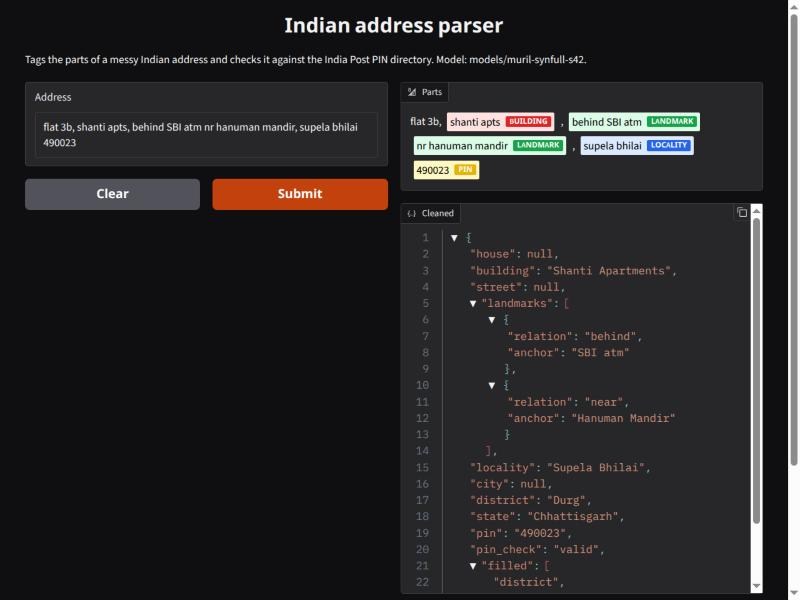
\includegraphics[width=0.80\textwidth]{figures/demo-muril.jpg}}
\caption{The demo running the MuRIL model on the first example.}\label{fig:demo}
\end{figure}

\section{Limitations}
\begin{enumerate}
\item \textbf{No large real test set.} The planned 500 human-written addresses were not collected, so RQ1 is
answered only on 20 addresses and RQ2 and RQ3 are not answered.
\item \textbf{hand20 is small and not independent.} 20 addresses give wide intervals, and the team wrote them and
used them while building the system.
\item \textbf{One training run.} MuRIL and \mbox{XLM-R} were trained with one seed; the plan asks for three.
\item \textbf{Label mappings.} The scores of the existing parsers depend on how we mapped their labels onto ours.
\item \textbf{Missing fields.} Our nine fields have no post office, police station, block or tehsil, which real
addresses in some states use often.
\item \textbf{Short name lists.} The generator uses short hand-written lists of place, landmark and building names.
\end{enumerate}

\section{Conclusion and future work}
We built a complete pipeline for studying how address parsers trained on synthetic data cope with real text: a data
generator with eight kinds of realistic noise, rules, a CRF and two fine-tuned transformers, a fair way to compare
them with existing parsers and a language model, a PIN checker, tools for collecting and labelling real addresses, and
a demo. The early evidence agrees with earlier work: models that are almost perfect on synthetic data lose 0.20 to
0.25 F1 on hand-written addresses, where simple rules do as well or better. Still, our systems beat every existing
open Indian address parser we tried.

\noindent{\sffamily\bfseries\color{brand}Next steps.}
\begin{enumerate}
\item Collect about 500 real public-place addresses with the form and label them, with two people checking 50.
\item Run the planned experiments: switch off each kind of noise in turn (RQ2), and add 25 to 200 real addresses to
the training data (RQ3), each with three seeds.
\item Add fields or rules for P.O., P.S., block and tehsil, and more real place names to the generator.
\end{enumerate}

\section{How to run it}
You need Python 3.12 and the \code{uv} tool. The model downloads itself from Hugging Face the first time (about
950\,MB).
\begin{lstlisting}
git clone https://github.com/devreddy1015/NLP_GROUP_PROJECT.git
cd NLP_GROUP_PROJECT
uv sync --extra train --extra demo
uv run python -m app.demo --model sandstromPL/muril-indian-address-parser
\end{lstlisting}
Then open \url{http://127.0.0.1:7860} and type an address. In the submitted project folder the model is already
included, so \code{-{}-model models/muril-synfull-s42} works without a download. Without uv,
\code{pip install -r requirements.txt} installs the same versions. The repository's README explains the other
commands.

\section*{Data and licences}
This work uses data from India Post: the All India Pincode Directory (data.gov.in), under the Government Open Data
Licence -- India (GODL-India). MuRIL and Qwen2.5 are released under Apache-2.0 and \mbox{XLM-R} under MIT; our fine-tuned
model is released under Apache-2.0.

% ======================= appendices =======================
\appendix

\section{Where the numbers come from}\label{app:runs}
\begingroup\raggedright\small
Every run writes \path{results/<run-id>.json} (and the predicted tags in \path{.pred.jsonl}); the tables in
\path{report/tables/} are built from these files by \path{scripts/make_tables.py}.
\begin{description}[style=nextline, leftmargin=1.5em, font=\sffamily\bfseries\color{brand}]
\item[Table~\ref{tab:main} and Table~\ref{tab:perlabel}] \path{20261110-rules-hand20-s0},
\path{20261110-crf-synfull-dev-s0}, \path{20261110-crf-synfull-hand20-s0}, \path{20261111-xlmr-synfull-dev-s42},
\path{20261111-xlmr-synfull-hand20-s42}, \path{20261116-muril-synfull-dev-s42}, \path{20261116-muril-synfull-hand20-s42}
\item[Table~\ref{tab:existing}] \path{20261111-shiprocket-indicbert-hand20-s0},
\path{20261111-shiprocket-tinybert-hand20-s0}, \path{20261111-mukuls-muril-hand20-s0},
\path{20261111-gagan-tinybert-hand20-s0}, \path{20261111-abr-parser-hand20-s0},
\path{20261111-l1-qwen-syn5shot-hand20-s42}, \path{20261111-l1-qwen-0shot-hand20-s42}
\item[Table~\ref{tab:compare}] \path{report/tables/shared.md}, built from the runs of Tables~\ref{tab:main}
and~\ref{tab:existing} and their \path{.pred.jsonl} files
\item[Table~\ref{tab:tuning}] \path{20261111-muril-synfull-dev-s42} and \path{-hand20-s42} (first try); the five
\path{20261111-muril-tune-*} runs on dev and hand20; \path{20261111-xlmr-synfull-dev-s42}; the two
\path{20261116-muril-synfull-*} runs
\item[Table~\ref{tab:pin}] \path{20261110-normalizer-synfull-dev-s0}, \path{20261110-normalizer-hand20-s0},
\path{20261116-muril-synfull-testcases20-s42}
\item[Section~\ref{sec:errors} and Appendix~\ref{app:stress}] \path{20261116-muril-synfull-hand20-s42.pred.jsonl}
against \path{tests/fixtures/handlabelled20.jsonl}, and
\path{20261116-muril-synfull-testcases20-s42.outputs.jsonl}
\end{description}
\endgroup

\clearpage
\section{Stress test: the result for each address}\label{app:stress}
The 20 addresses are in \code{indian\_address\_parser\_test\_cases.md}; the model's full output is in
\code{report/test\_cases\_output.md}. ``PIN tagged'' is the text MuRIL tagged as the PIN; the last column lists the
fields it tagged, with a count when a field was tagged more than once.

\begin{table}[H]
\centering\small
\caption[Stress test: the result for each address]{MuRIL and the PIN check on the 20 test addresses.}\label{tab:stress}
\begin{tabularx}{\textwidth}{@{}lllL@{}}
\toprule
\textbf{Case} & \textbf{PIN tagged} & \textbf{PIN check} & \textbf{Fields tagged}\\
\midrule
REAL-01 & 722101 & valid & LOCALITY $\times$2, CITY, BUILDING, STREET, DISTRICT, PIN\\
REAL-02 & 722122 & valid & CITY, BUILDING, LOCALITY, DISTRICT, PIN\\
REAL-03 & 713101 & mismatch & BUILDING, STREET, LOCALITY, DISTRICT, PIN\\
REAL-04 & 733141 & mismatch & LANDMARK, LOCALITY $\times$5, STATE $\times$2, DISTRICT, PIN\\
REAL-05 & 733133 & mismatch & STREET, LOCALITY $\times$2, CITY $\times$3, STATE $\times$3, DISTRICT, PIN\\
REAL-06 & 733124 & mismatch & LANDMARK, LOCALITY $\times$2, CITY $\times$3, DISTRICT, STATE, PIN\\
REAL-07 & 16 & not found & HOUSE, STREET $\times$2, LOCALITY $\times$4, CITY, PIN\\
REAL-08 & 700043 & mismatch & HOUSE, STREET, CITY $\times$2, PIN, STATE $\times$4, LOCALITY $\times$3, LANDMARK\\
REAL-09 & 700024 & mismatch & CITY, PIN, STATE $\times$2, LOCALITY $\times$3, LANDMARK\\
REAL-10 & 700070 & valid & LOCALITY $\times$3, CITY, PIN, LANDMARK\\
REAL-11 & 834002 & mismatch & HOUSE, STREET $\times$2, CITY $\times$4, PIN $\times$3, LOCALITY $\times$7, LANDMARK
$\times$3, STATE, DISTRICT\\
REAL-12 & 815302 & mismatch & LOCALITY $\times$4, STREET, CITY $\times$2, STATE $\times$3, DISTRICT, PIN\\
REAL-13 & 783385 & valid & CITY, STREET, BUILDING, LOCALITY $\times$2, DISTRICT, STATE, PIN\\
\midrule
SYN-14 & 000000 & not found & BUILDING $\times$2, HOUSE, STREET $\times$2, LANDMARK $\times$2, LOCALITY $\times$3,
DISTRICT, STATE, PIN\\
SYN-15 & 123456 & not found & BUILDING, HOUSE, STREET $\times$3, LOCALITY $\times$5, LANDMARK $\times$2, CITY
$\times$2, DISTRICT, STATE, PIN\\
SYN-16 & 999999 & not found & HOUSE $\times$2, STREET $\times$2, LANDMARK $\times$4, LOCALITY $\times$2, CITY,
DISTRICT, STATE, PIN\\
SYN-17 & 111111 & not found & LANDMARK $\times$3, LOCALITY $\times$4, CITY $\times$2, DISTRICT, STATE, PIN\\
SYN-18 & 5600O1 & not found & HOUSE, BUILDING, STREET, LANDMARK $\times$3, LOCALITY, DISTRICT, STATE, PIN\\
SYN-19 & 500000 & not found & BUILDING, LOCALITY $\times$4, STREET $\times$2, LANDMARK $\times$3, DISTRICT, STATE,
PIN\\
SYN-20 & 765432 & not found & HOUSE $\times$2, LOCALITY $\times$2, DISTRICT $\times$2, PIN $\times$2, BUILDING,
STREET, LANDMARK, STATE\\
\bottomrule
\end{tabularx}
\end{table}
REAL = a real public-office address; SYN = an invented hard case. In REAL-11 the PIN was tagged three times because
the address writes 834002 three times; in SYN-20 it was tagged twice because two addresses are pasted together.

\begin{thebibliography}{99}
\raggedright
\bibitem{etasr} Dhavase and Chaudhary. Improving Indian address parsing in data-scarce environments using chunk-based
retrieval-augmented transformer models. \emph{Engineering, Technology \& Applied Science Research}, 2026.
\url{https://doi.org/10.48084/etasr.18510}
\bibitem{indiapost} India Post. All India Pincode Directory. data.gov.in.
\url{https://www.data.gov.in/catalog/all-india-pincode-directory}
\bibitem{muril} Khanuja et al. MuRIL: Multilingual representations for Indian languages, 2021.
\url{https://huggingface.co/google/muril-base-cased}
\bibitem{xlmr} Conneau et al. Unsupervised cross-lingual representation learning at scale (\mbox{XLM-R}). ACL, 2020.
\url{https://huggingface.co/FacebookAI/xlm-roberta-base}
\bibitem{qwen} Qwen Team. Qwen2.5-1.5B-Instruct. \url{https://huggingface.co/Qwen/Qwen2.5-1.5B-Instruct}
\bibitem{shiprocket} Shiprocket AI. Open IndicBERT and TinyBERT Indian address NER models.
\url{https://huggingface.co/shiprocket-ai}
\bibitem{mukuls} mukuls9971. MuRIL Indian address NER v1.
\url{https://huggingface.co/mukuls9971/muril-indian-address-ner-v1}
\bibitem{gagan} gagan1985. TinyBERT Indian address parser.
\url{https://huggingface.co/gagan1985/tinybert-4l-312d-indian-address-parser}
\bibitem{abr} abr-6024. Indian address parser 1.5B. \url{https://huggingface.co/abr-6024/indian-address-parser-1.5B}
\bibitem{deepparse} Yassine et al. Leveraging subword embeddings for multinational address parsing (deepparse), 2020.
\url{https://arxiv.org/abs/2006.16152}
\bibitem{geoindia} Singhal et al. GeoIndia: a seq2seq geocoding approach for Indian addresses. EMNLP Industry
Track, 2024. \url{https://aclanthology.org/2024.emnlp-industry.29.pdf}
\bibitem{seqeval} seqeval: a Python framework for sequence labelling evaluation.
\url{https://github.com/chakki-works/seqeval}
\bibitem{ours} Our model on Hugging Face: \url{https://huggingface.co/sandstromPL/muril-indian-address-parser}
\end{thebibliography}

\end{document}
